%----------------------------------------------------------------------------------------
%	PACKAGES AND OTHER DOCUMENT CONFIGURATIONS
%----------------------------------------------------------------------------------------

\documentclass[paper=a4, fontsize=11pt, oneside]{scrartcl} % A4 paper and 11pt font size

\usepackage[T1]{fontenc} % Use 8-bit encoding that has 256 glyphs
\usepackage{fourier} % Use the Adobe Utopia font for the document - comment this line to return to the LaTeX default
\usepackage[english]{babel} % English language/hyphenation
\usepackage{amsmath,amsfonts,amsthm} % Math packages

\usepackage{lipsum} % Used for inserting dummy 'Lorem ipsum' text into the template

\usepackage{sectsty} % Allows customizing section commands
\allsectionsfont{\centering \normalfont\scshape} % Make all sections centered, the default font and small caps

\usepackage{rotating} % Used for sidewaysfigure and other rotation options.

\usepackage[parfill]{parskip}

\usepackage{fancyhdr} % Custom headers and footers
\pagestyle{fancyplain} % Makes all pages in the document conform to the custom headers and footers
\fancyhead{} % No page header - if you want one, create it in the same way as the footers below
\fancyfoot[L]{} % Empty left footer
\fancyfoot[C]{} % Empty center footer
\fancyfoot[R]{\thepage} % Page numbering for right footer
\renewcommand{\headrulewidth}{0pt} % Remove header underlines
\renewcommand{\footrulewidth}{0pt} % Remove footer underlines
\setlength{\headheight}{13.6pt} % Customize the height of the header

\usepackage{graphicx} % Allows the use of images in the document
\graphicspath{ {images/} } % Instructs LaTeX to search the 'images' directory for images.

%\numberwithin{equation}{section} % Number equations within sections (i.e. 1.1, 1.2, 2.1, 2.2 instead of 1, 2, 3, 4)
%\numberwithin{figure}{section} % Number figures within sections (i.e. 1.1, 1.2, 2.1, 2.2 instead of 1, 2, 3, 4)
%\numberwithin{table}{section} % Number tables within sections (i.e. 1.1, 1.2, 2.1, 2.2 instead of 1, 2, 3, 4)

\setlength\parindent{0pt} % Removes all indentation from paragraphs - comment this line for an assignment with lots of text

%----------------------------------------------------------------------------------------
%	TITLE SECTION
%----------------------------------------------------------------------------------------

\newcommand{\horrule}[1]{\rule{\linewidth}{#1}} % Create horizontal rule command with 1 argument of height

\title{	
\normalfont \normalsize 
\textsc{Concordia University} \\
\textsc{Department of Computer Science and Software Engineering} \\
\textsc{SOEN 341/4 S \qquad Software Process \qquad Winter 2016} \\ [25pt] % University, school and/or department name(s)
\horrule{0.5pt} \\[0.4cm] % Thin top horizontal rule
\huge Mytinerary: \\ System Overview and Team Members \\ % The assignment title
\horrule{2pt} \\[0.5cm] % Thick bottom horizontal rule
}

\author{Group Member Names} % Names

\date{\normalsize January 13, 2016} % Date

\begin{document}

\maketitle % Print the title

%----------------------------------------------------------------------------------------
%	SYSTEM OVERVIEW
%----------------------------------------------------------------------------------------

\section*{System Overview}
The name of our system is Mytinerary.

The system will be used to generate all possible multi-year schedules for a Concordia student.
The number of possible schedules are determined based on three criteria: the student's preferences, courses taken, and academic record.

The system can then use a student's academic record to determine the program requirements for the student.
The system then uses a list of courses completed by the student to determine which prerequisites the student has, and which courses they must take.
Finally, the user can set preferences for their schedule, for example: preferred course load, times available and desired graduation date.

Based off these three criteria, Mytinerary will output all possible  multi-year schedules for the student.

Mytinerary only contains two user classes: the student, who can set their preferences and request schedules; and the program director, who can view and edit the academic record of any student in their respective program, and can modify course section details.
\begin{figure}[H]
\centering
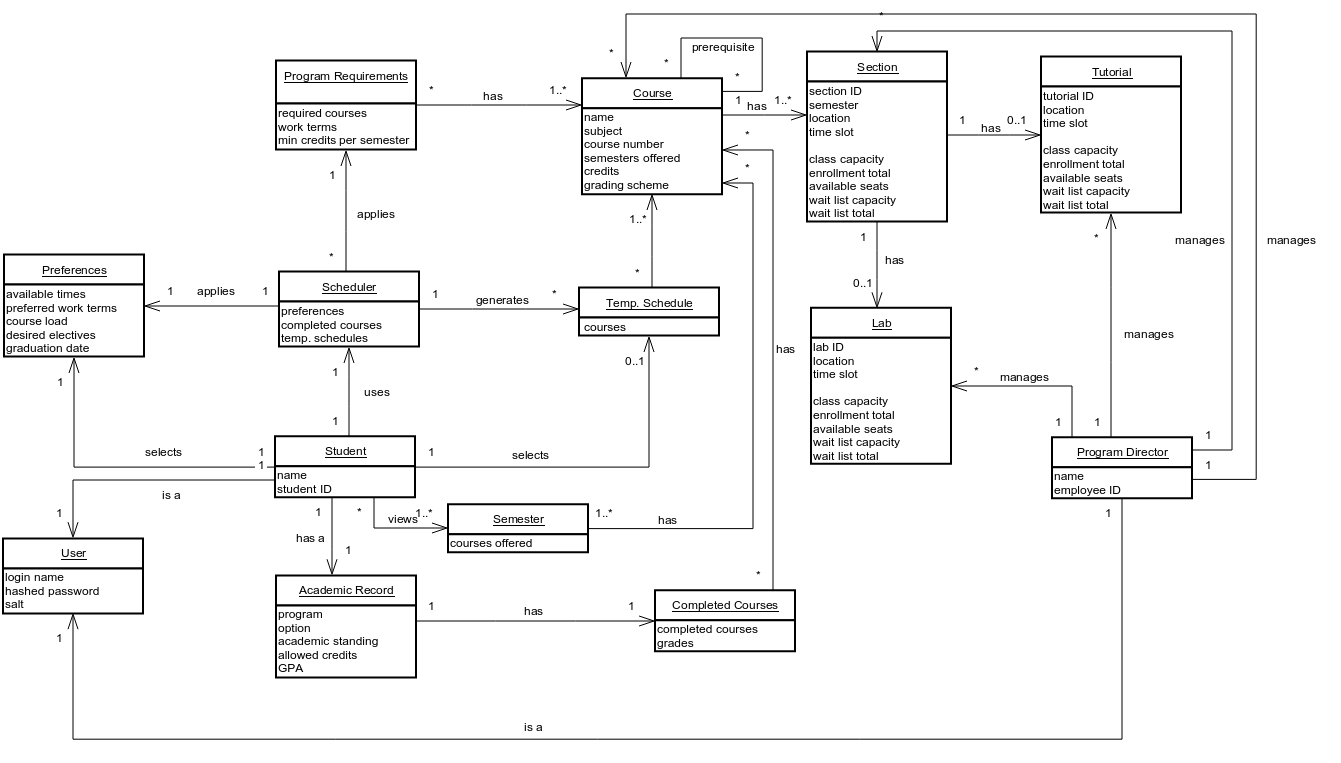
\includegraphics[width=1.4\textwidth, angle=-90]{domain_model}
\caption{Domain Model for Mytinerary}
\label{fig:DM}
\end{figure}

%----------------------------------------------------------------------------------------
%	TEAM MEMBERS
%----------------------------------------------------------------------------------------
\newpage
\section*{Team Members}

\end{document}
